\section*{\color{olive}Ejercicio 3: Simulaci\'on de la respuesta en frecuencia de un circuito en condiciones iniciales}

Durante este ejercicio se procedi\'o a simular el circuito de la Figura
\ref{circ3}. Se nos pidi\'o obtener el tipo de singularidad del circuito,
a qu\'e elemento reactivo se asociaba, y el valor asociado a ese elemento. 

\begin{figure}[H] %!ht 
 \begin{center}
    \begin{circuitikz}[american]
    \draw (0,3) to[V,v=$V_{AC}$] (0,1.5)to[V,v=$V_{DC}$] (0,0) % The voltage sources
(0,3) to[R, R=$R_G$] (2,3)  to[R, R=$R$] (4,3)  node[anchor=west] {OUT} 
(4,0) to[Do] (4,3)
(4,0) to[short] (0,0)
(2,0) node[ground]{}
(2,3) node[anchor=south] {IN} 
;
    \end{circuitikz}
    \caption{Circuito empleado para medir la curva caracter\'istica de un diodo.}
\label{circ3}
\end{center}
\end{figure}

Siendo $R = 200k\Omega$. \\ 

Al realizar la simulaci\'on, se obtuvo un Bode como
el que se puede ver en la figura \ref{b_3}.


\begin{figure}[H]
\begin{centering}
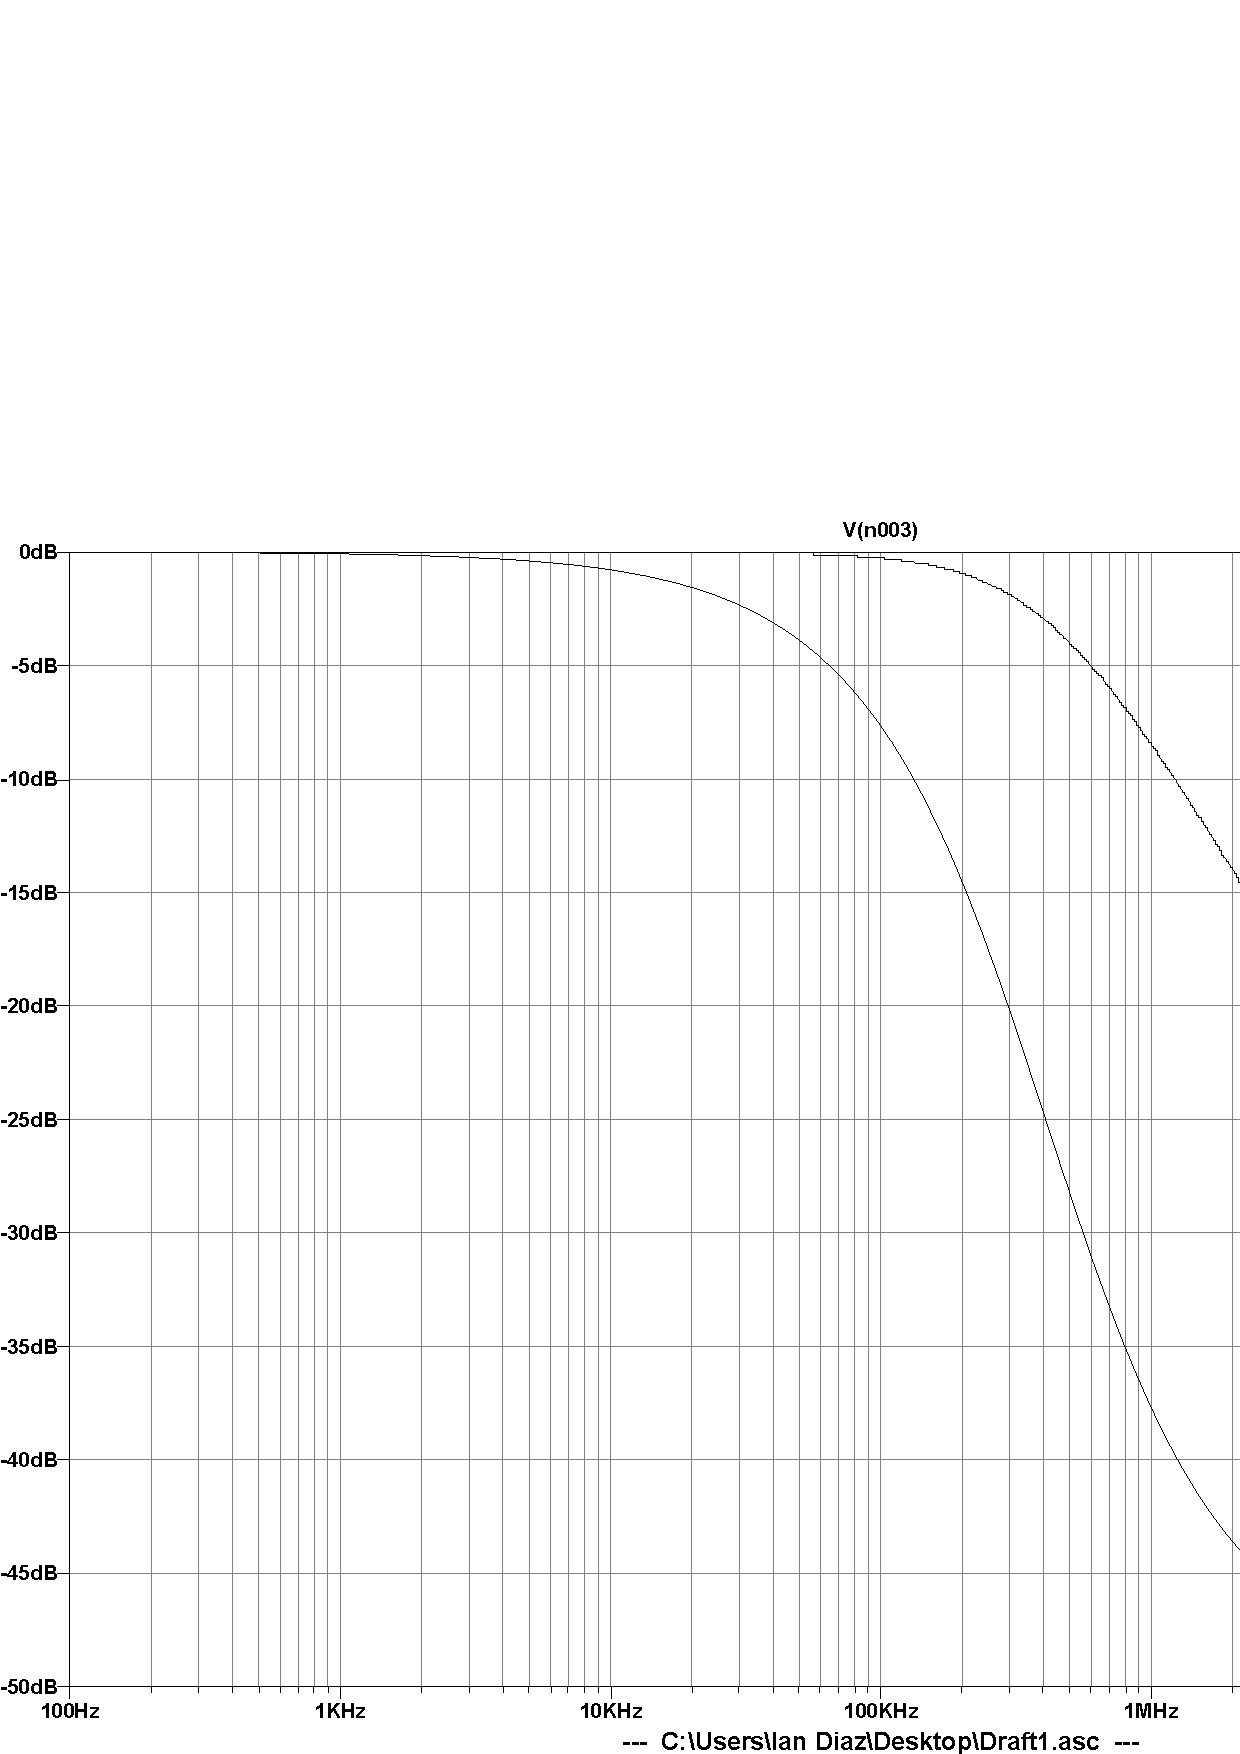
\includegraphics[scale=0.25]{../EJ3/Bode}
\par\end{centering}
\caption{Bode}
\label{b_3}
\end{figure}

Viendo el diagrama de Bode de la figura \ref{b_3}, sabiendo que la amplitud es
la l\'inea negra y la fase la l\'inea gris, podemos determinar que se
comporta como un filtro pasabajos y la singularidad es un polo, ya que la fase cae 90\textdegree .
Por lo tanto, podemos decir que el diodo a altas frecuencias se comporta
como un capacitor. Luego de ver este comportamiento, buscamos la hoja
de datos del 1N4148 y se encontr\'o que la capacidad total del diodo
es de 4(pF), sin embargo, como se puede ver en la figura \ref{b2_3},
el diagrama de bode no coincide completamente con el del circuito de la figura
\ref{circ3}. Para que coincida perfectamente, debemos usar un capacitor
de aproximadamente 2(pF). Creemos que la diferencia de capacidad entre
el valor obtenido en la hoja de datos y el calculado, se debe a un
modelo equivalente del diodo que no coincide exactamente con el
de la realidad, generando pequeñas diferencias, como la mencionada.

\begin{figure}[H]
\begin{centering}
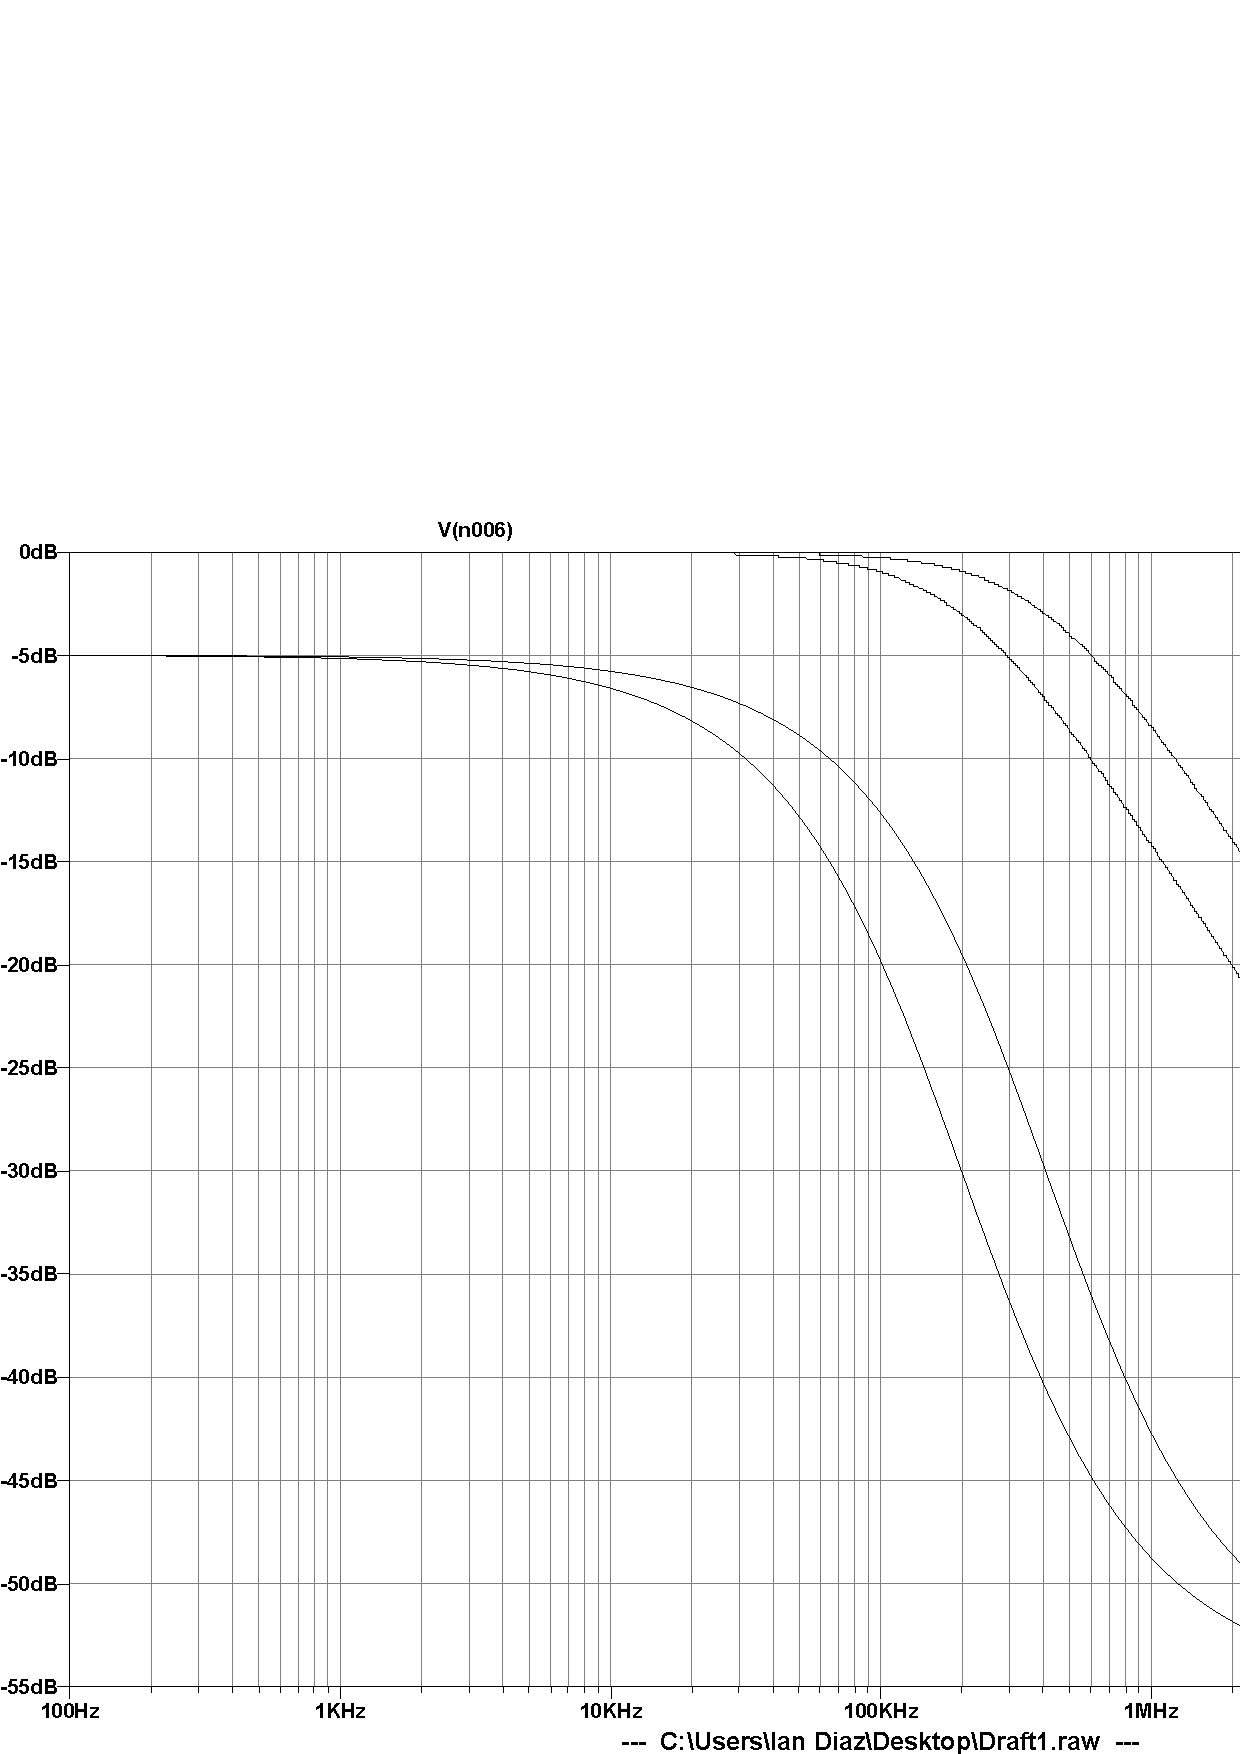
\includegraphics[scale=0.2]{../EJ3/Bode2}
\par\end{centering}
\caption{Bode Diodo vs Capacitor nominal}
\label{b2_3}
\end{figure}










